\newpage
\section{Aufbau und Durchführung}
\label{sec:Durchführung}

%\subsection{Justage}
%Zu Beginn ist eine Justierung des Interferometers notwendig.
%Ziel ist eine Aufspaltung eines Strahls in zwei Strahlen, die beide in
%der horizontalen Ebene liegen und anschließendes Überlappen der Strahlen
%beim Verlassen des Interferometers. Dies wird durch Einstellen der
%Spiegel innerhalb und außerhalb des Interferometers erreicht.


\subsection{Messung des Kontrasts}
Zur Messung des Kontrasts wird ein linearer Polarisationsfilter mit $45\si{\degree}$
Ausrichtung verwendet, der hinter dem PBSC positioniert wird.
Dadurch entsteht ein Interferenzbild, dessen Intensität durch eine Photodiode gemessen wird.
Nun wird der Winkel des ersten Polarisationsfilters variiert
und die Glasplättchen so rotiert, dass zum einen ein Intensitätminimum und zum anderen
ein Intensitätsmaximum gemessen werden kann.

\subsection{Bestimmung der Brechungsindices}
Für die Bestimmung der Brechungsindices wird der
Winkel des ersten Polarisationsfilters so gewählt, dass ein Kontrastmaximum vorliegt.
Weiterhin werden der zweite Polarisationsfilter entfernt.
Stattdessen trifft der gebündelte Strahl auf einen Polarisationsseperator, realisiert durch einen
weiteren PBSC und einen Spiegel, wie in Abbildung \ref{fig:polsep} zu sehen.
\begin{figure}
     \centering
     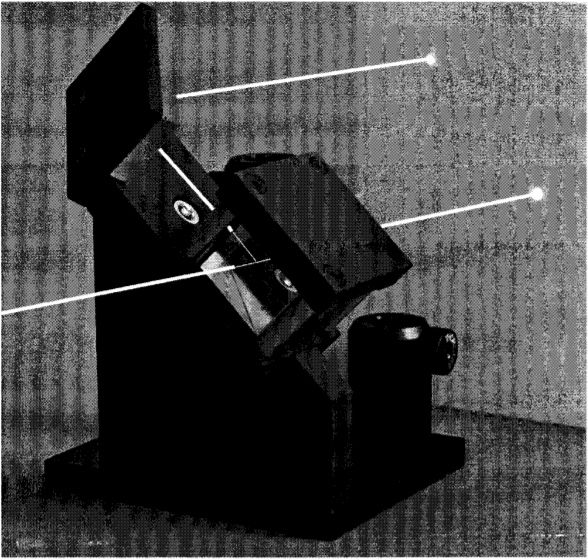
\includegraphics[width=0.5\textwidth]{PSBC.PNG}
     \caption{Aufbau des Polarisationsseperator.\cite{skript}}
     \label{fig:polsep}
\end{figure}
\FloatBarrier
Mittels zweier Photodioden wird der zuvor aufgespaltene Strahl detektiert.
Mit einem Oszilloskop wird die Spannungsdifferenz zwischen den Intensitäten
gemessen. Ein weiteres Gerät zählt die Nulldurchgänge der Spannungsdifferenz.
Bei der Messung für den Brechungsindex von Glas wird
der Winkel der Glasplättchen langsam verändert und die Nulldurchgänge für unterschiedliche
Winkel aufgenommen.

Für den Brechnungsindex von Luft werden die Glasplättchen
aus dem Strahlengang entfernt. Es wird eine Gaszelle eingebaut, durch
die nur ein Laserstrahl geht. Die Gaszelle ist verbunden mit einer Pumpe,
die ein Vakuum in der Gaszelle erzeugt. Durch ein Ventil wird wieder langsam
Luft in die Zelle gelassen bis der Normaldruck erreicht ist. Während
dieses Vorganges werden wieder Nulldurchgänge von der Spannungsdifferenz aufgenommen.
